\documentclass{article}

% Language setting
% Replace `english' with e.g. `spanish' to change the document language
\usepackage[english]{babel}
\usepackage[utf8]{inputenc}
% Set page size and margins
% Replace `letterpaper' with`a4paper' for UK/EU standard size
\usepackage[letterpaper,top=2cm,bottom=2cm,left=3cm,right=3cm,marginparwidth=1.75cm]{geometry}

% Useful packages
\usepackage{kotex}
\usepackage{amsmath}
\usepackage{amsfonts}
\usepackage{amssymb}
\usepackage{graphicx}
\usepackage{amsthm}
\usepackage[sorting=none]{biblatex}
\usepackage{subcaption}
\addbibresource{sample.bib}
% \usepackage[colorlinks=true, allcolors=blue]{hyperref}
\newtheorem{lemma}{Lemma}
\newtheorem*{prop}{Proposition}
\newtheorem*{theorem}{Theorem}
\newtheorem*{definition}{Definition}
\newtheorem*{corol}{Corollary}
\newtheorem*{remark}{Remark}
\newtheorem*{example}{Example}
\newtheorem*{claim}{Claim}
\newtheorem{fact}{Fact}
\newcommand{\tr}[1]{
\textrm{tr}(#1)}
\newcommand{\red}[1]{
\color{red}
#1
\color{black}
}
\newcommand{\Z}{\mathbb{Z}}
\newcommand{\Q}{\mathbb{Q}}
\newcommand{\R}{\mathbb{R}}
\newcommand{\C}{\mathbb{C}}
\newcommand{\B}{\mathbb{B}}
\newcommand{\ra}{\Rightarrow}
\newcommand{\cyclic}[1]{\left\langle #1\right\rangle}
\newcommand{\im}{\textrm{im}}

\renewcommand{\labelitemii}{$\bullet$}
\renewcommand{\iff}{\Leftrightarrow}
\title{Advances in Convolutional Neural Networks\\Programming Assignment}
\author{20233611 Hojun Lee}
\begin{document}
\maketitle

\section{Knowledge Distillation}
In general, larger and deeper models in classification tasks are expected to have better performance. However, there are some situations in which memory usage is restricted or requires immediate predictions. It would be admirable if a smaller and simpler model achieves a similar performance to a bigger and deeper model. If a pre-trained larger and deeper model (teacher model) can transfer knowledge to a smaller and simpler model (student model), it would be more helpful than the student model training alone.\\

Then, how can we define knowledge? When we use a neural network in a classification task, we often add a softmax layer at the end of the layer to let the logit $z_i$ mean the probability of the input belonging in the $i$th class.
\begin{equation}
    p_i=\frac{exp(z_i)}{\sum\limits_jexp(z_j)}
\end{equation}
And then, the model predicts the class that has the greatest probability as the answer. If a class has a slightly big probability (e.g. $p=0.1$) even if it is not an accurate class, we can expect that there are some similar properties between the class and the accurate class. Otherwise, it means that the class has completely different properties to the accurate class. Hinton considered the probabilities of other classes as knowledge. \cite{hinton2015distilling} Since the probabilities are too small to use for training, he softened the probability as the following.
\begin{equation}
    q_i=\frac{exp(z_i/T)}{\sum\limits_jexp(z_j/T)}
\end{equation}
Here, $T$ is called a temperature.\\

We use a weighted sum of two losses, the original loss, which is a cross-entropy loss between student output and the label, and a Kullback–Leibler divergence between soft targets of the student and teacher model. Since the magnitude of a gradient of the Kullback-Leibler divergence of softened targets scales $1/T^2$, let's multiply $T^2$ for this loss. The object function is 
\begin{equation}
    \mathcal{L}=\mathcal{L}_{CE}(p_s,y)+\lambda T^2\mathcal{L}_{KL}(q_s,q_t),
\end{equation}
where $p_s$ is the output probability of the student model, and $q_s,q_t$ are softened output probability of the student model and the teacher model, respectively.
\section{Training Process}
\subsection{Training algorithm implementation}
I divided the training data into \texttt{batch\_size=64} data and optimized the cost function for each minibatch. Figure \ref{fig:loss-code} is the code that implements a training process for a single minibatch.

\begin{figure}[h!]
    \centering
    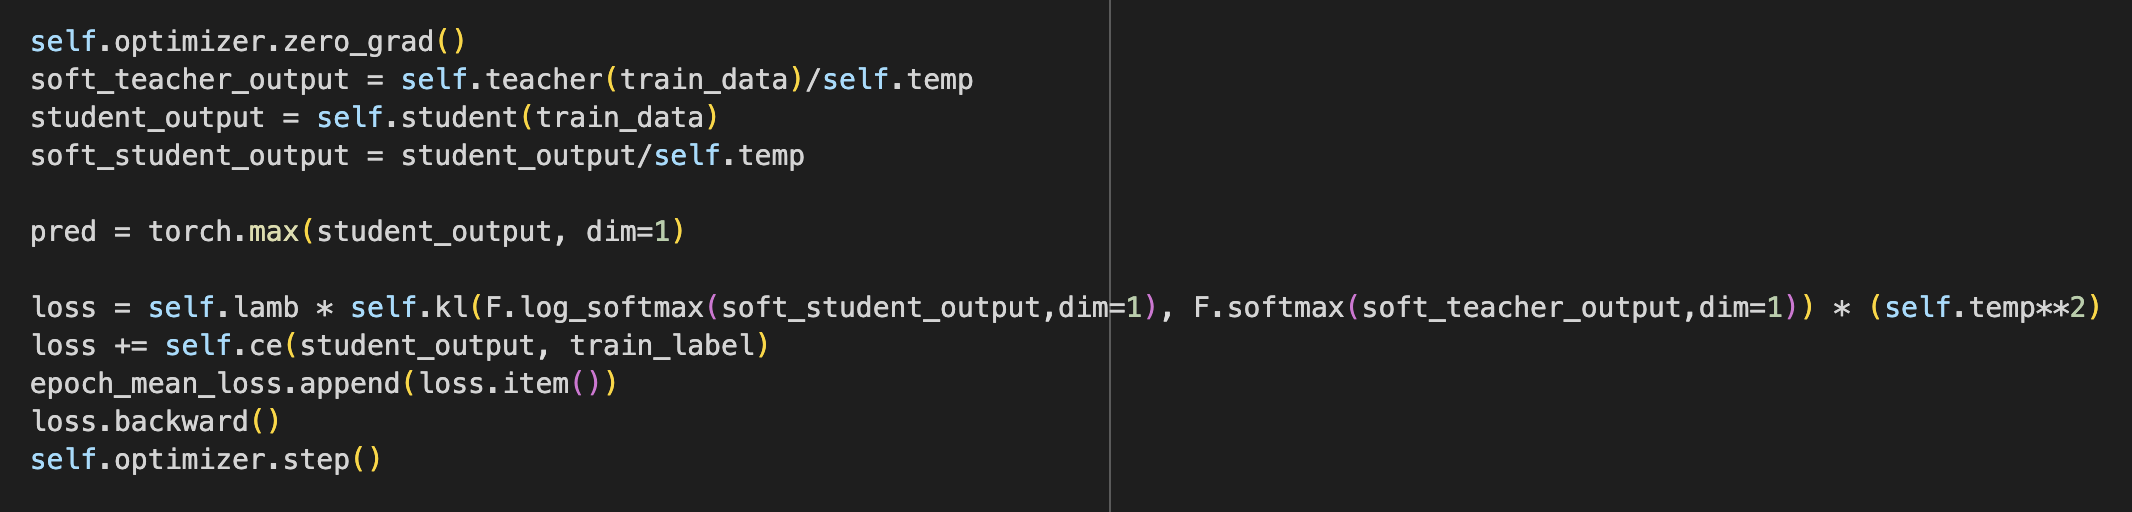
\includegraphics[width=\textwidth]{loss-code.png}
    \caption{Training process for a single minibatch. Since \texttt{KLDivLoss} method in PyTorch is defined as \texttt{loss\_pointwise = target * (target.log() - input)}, we have to apply log function to the input.}
    \label{fig:loss-code}
\end{figure}

\subsection{Hyperparameter search}

For hyper-parameter search, I used Adam optimizer with \texttt{lr=1e-3, betas=(0.9,0.999), weight\_decay = 1e-4}. I used a random search with a log-uniform distribution (See Figure \ref{fig:sample-hyp-code} for details) rather than using a grid search. \cite{bergstra2012random}
I compared the test accuracy for each hyper-parameter combination after 30 epochs.

\begin{figure}[h!]
    \centering
    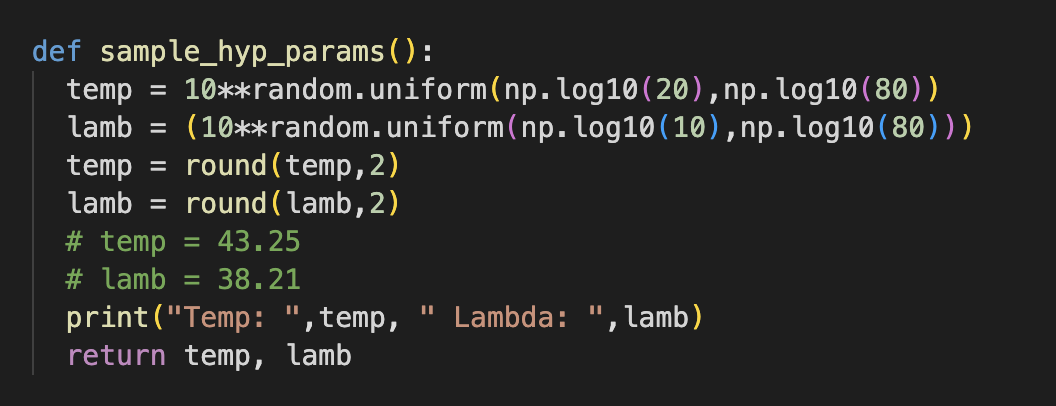
\includegraphics[width=0.6\textwidth]{sample_hyp-code.png}
    \caption{A code for sampling hyper-parameters. Initially, \texttt{temp} and \texttt{lamb} are sampled log-uniformly between $10^{0}\sim 10^{2}$ and $10^{-2}\sim 10^{2}$, respectively, and then refine the scope to the region where the test accuracy is high. }
    \label{fig:sample-hyp-code}
\end{figure}

\begin{figure}[h!]
    \centering
    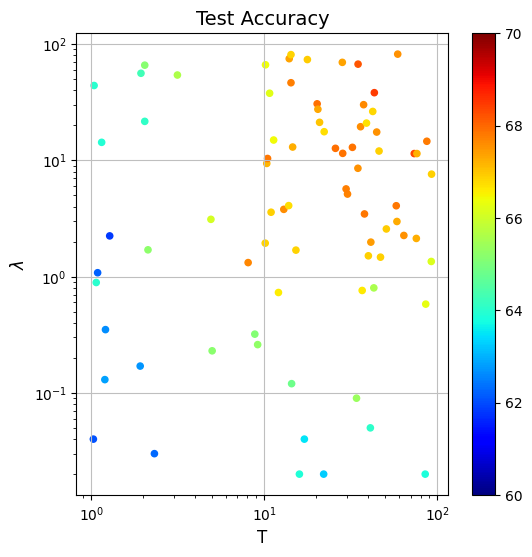
\includegraphics[width=200pt]{hyp.png}
    \caption{Test accuracy for various temperature $T$ and $\lambda$ in percent.}
    \label{fig:hyp-param-plot}
\end{figure}
The hyper-parameter combination that achieves the highest test accuracy was $T=43.25$, $\lambda=38.21$, and it achieved a test accuracy of $68.44\%$.
\subsection{Train}
For actual training, I used hyper-parameters $T=43.25$, $\lambda=38.21$ that I found, and Adam optimizer with \texttt{lr=1e-3, betas=(0.9,0.999), weight\_decay = 1e-4} for 180 epochs. And then, I reduced the learning rate to \texttt{1e-4} and trained 20 additional epochs.

\section{Result}

Figure \ref{fig:result} shows the loss, training accuracy, and test accuracy for the training process.

\begin{figure}[h!]
\centering
\begin{subfigure}[b]{0.45\textwidth}
    \centering
    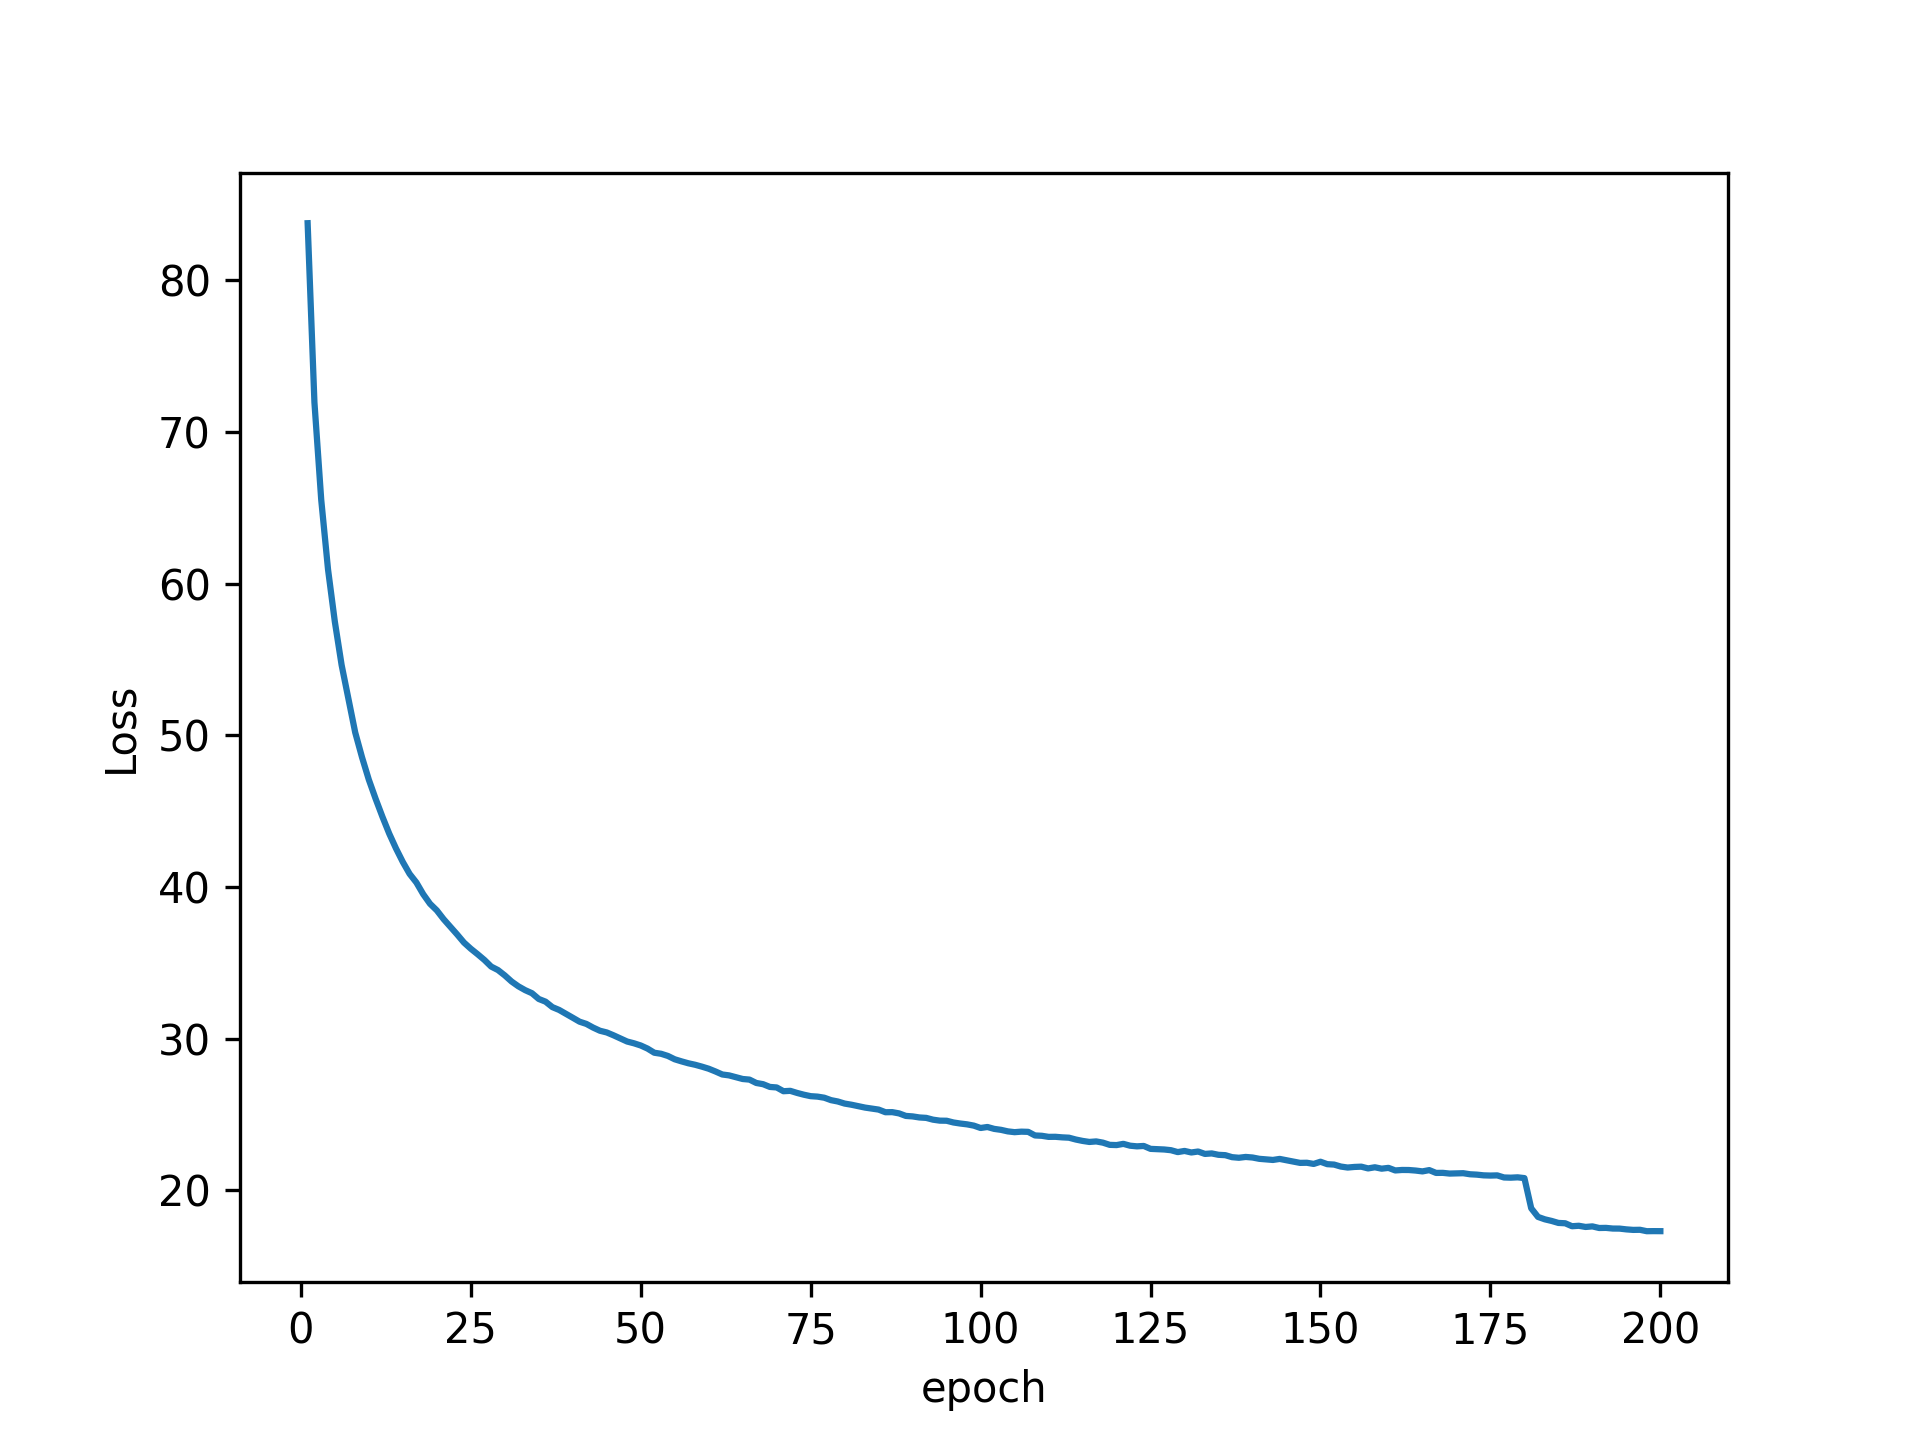
\includegraphics[width=\textwidth]{loss.png}
    \caption{Loss plot for 200 epochs}
\end{subfigure}
\begin{subfigure}[b]{0.45\textwidth}
    \centering
    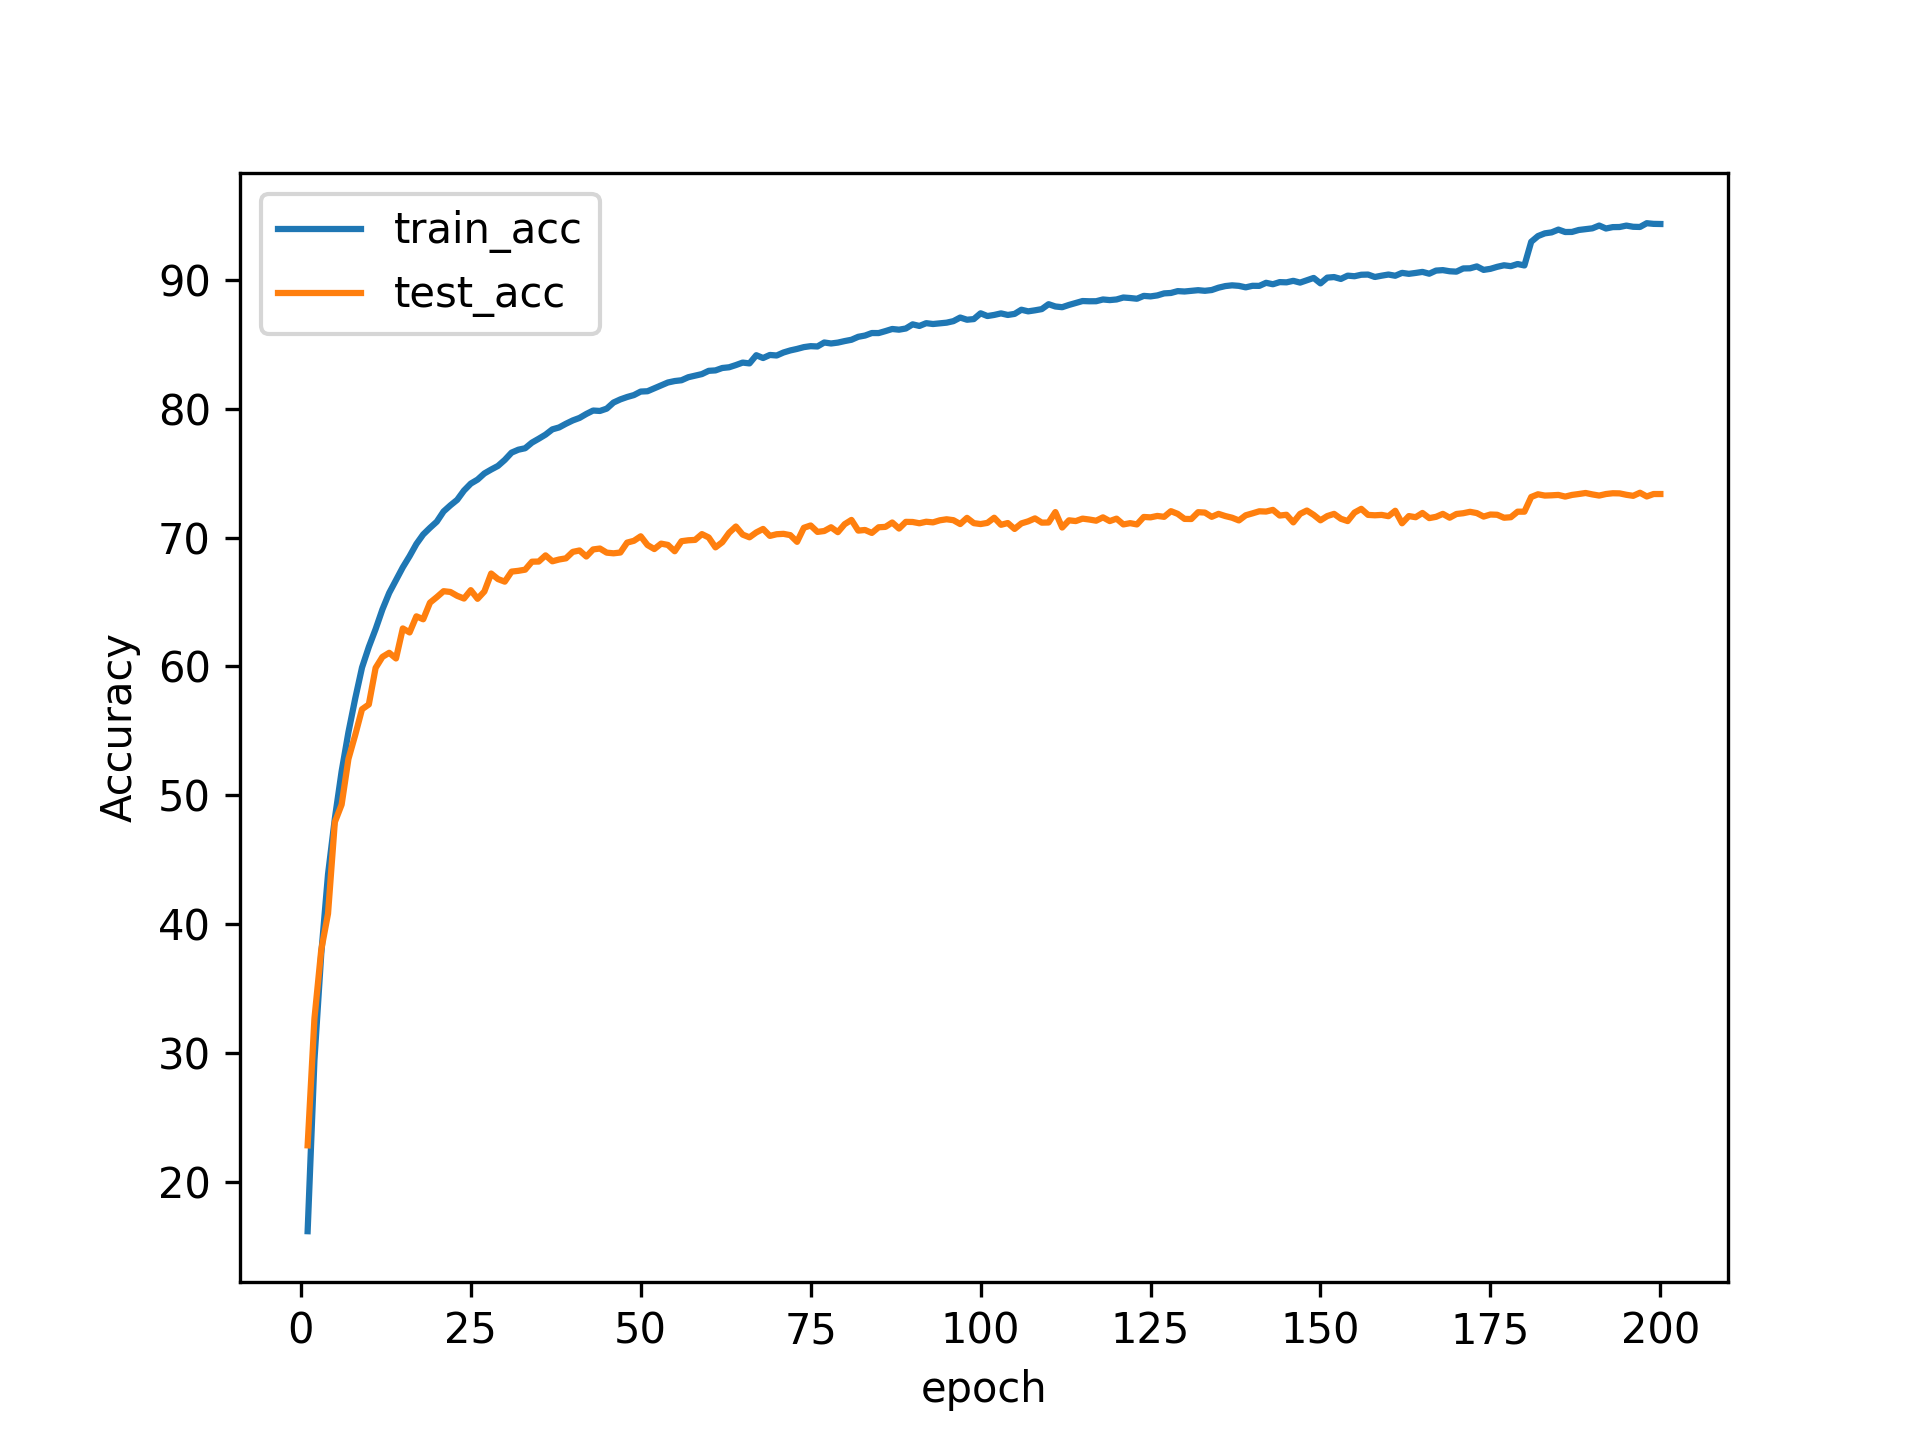
\includegraphics[width=\textwidth]{acc.png}
    \caption{Training and test accuracy for 200 epochs}
\end{subfigure}
\caption{Plot of loss, training accuracy, and test accuracy.}
\label{fig:result}
\end{figure}



The final test accuracy was 73.380\%.

\begin{figure}[h!]
    \centering
    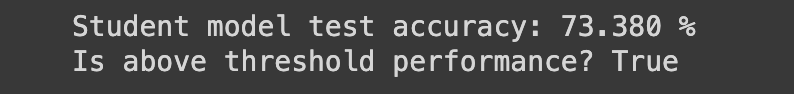
\includegraphics[width=0.6\textwidth]{fin_acc.png}
\end{figure}
\printbibliography
\end{document}